\documentclass[10pt]{article}


\usepackage[en-US]{datetime2}

\usepackage{fontspec}

\usepackage{caption}

\usepackage{amsmath} \allowdisplaybreaks

\usepackage[luatex]{graphicx} \ifdefined \setgraphicspath \setgraphicspath \fi

\usepackage{xcolor} \definecolor{gold}{RGB}{255, 180, 0} \definecolor{purp}{RGB}{180, 0, 255}

\usepackage[export]{adjustbox}

\usepackage{varioref}

\usepackage[colorlinks=false, pdfborder={2 2 2}, linkbordercolor=gold, urlbordercolor=gold, citebordercolor=purp]{hyperref}

\usepackage{cleveref}

\usepackage[all]{hypcap}

\usepackage{moreverb}

\usepackage{csagh}


\renewcommand\figurename {Figure}

\renewcommand\tablename  {Table}

\renewcommand\refname    {References}


\def\listingoffset{\leftmargini}

\def\listinglabel#1{\rlap{\footnotesize\sffamily\the#1}\hskip\listingoffset{}\relax}


\def\AAAB{\textit{A15}}

\def\TS{Tetrastix} \def\TSP{Tetrastix~Prism} \def\TTSp{The~Tetrastix~prism} \def\tTSp{the~Tetrastix~prism}

\def\WP{Weaire--Phelan} \def\WPH{Weaire--Phelan~Honeycomb} \def\TWPh{The~Weaire--Phelan~honeycomb}
\def\tWPh{the~Weaire--Phelan~honeycomb}

\def\IL{Infima~Labs} \def\il{infimalabs}


\begin{document}


\received{\DTMDisplaydate{2023}{10}{3}{-1}} \revised{\today}


\begin{opening}


  \author[ \IL, \URL{https://\il.com}, e-mail: \URL{anthony@\il.com}\\ Snap Game Services, \URL{https://snap.gs}, e-mail:
  \URL{anthony@snap.gs} ]{ C Anthony Risinger }


  \title{ \emph{Accelerating} {\normalsize the} Virtual Experience\newline{} {\normalsize via} Compactification {\normalsize of
  the} Metaverse }


  \begin{abstract}

    \setlength{\parindent}{0em}

    Spatial computing stands at the heart of immersive, competitive experiences. When reality yields to fast-paced virtual
    arenas, every millisecond can clutch the win, and every dropped frame can shatter the illusion. Widespread spatial
    partitioning of different virtual realities (VR) with the topologically close-packed \textbf{\AAAB{} phase structure}
    ($\beta$--$W$) promises to thread new, scalable dimensions of isotropic order into the fabric of the metaverse itself.

    \setlength{\parskip}{1em}

    This research advances the development of a~trans-metaversal coordination space. Latency-sensitive, full-body VR
    experiences---such as online multiplayer tournaments---are close to insufferable under the current infrastructure. In lieu of
    a~shared, compact spatial representation, downstream spatial protocols resort to resharing the original floating-point
    coordinates. Full immersion demands tenfold the coordinates at double the speed---simply relaying the positional coordinates
    of a~5-on-5 full-body VR match can exceed 100 kbps per user.

    The proposed solution rounds each three-dimensional (3D) floating-point coordinate---and all its unused dynamic range---to
    the nearest \AAAB{}-encoded integer representation, one or more dimensions higher. It centers \AAAB{} inside \tWPh{}, or
    \tTSp{}, then equally discretizes all 3D floating-point space. The result is a~numerically-stable, higher-order space that's
    packable, stackable, and less than half the size in memory---assigning each high-dimensional coordinate to a~consistent
    volume of 3D space shrinks the encoding of nearby coordinates, minimizes directional aliasing, and maintains compatibility
    with global measurement standards.

    In a~quest for instant replay and deterministic fidelity, aligning virtualities with \AAAB{} ensures every bit of space is
    part of the living, responsive experience.

  \end{abstract}


  \keywords{ \AAAB, Beta-Tungsten, Competitive Virtual Reality, Metaverse, Numeric Stability, Pm-3n, Spatial Computing, \TSP,
  \WPH, \emph{\IL} }


\end{opening}


\begin{figure}[!ht]\capstart 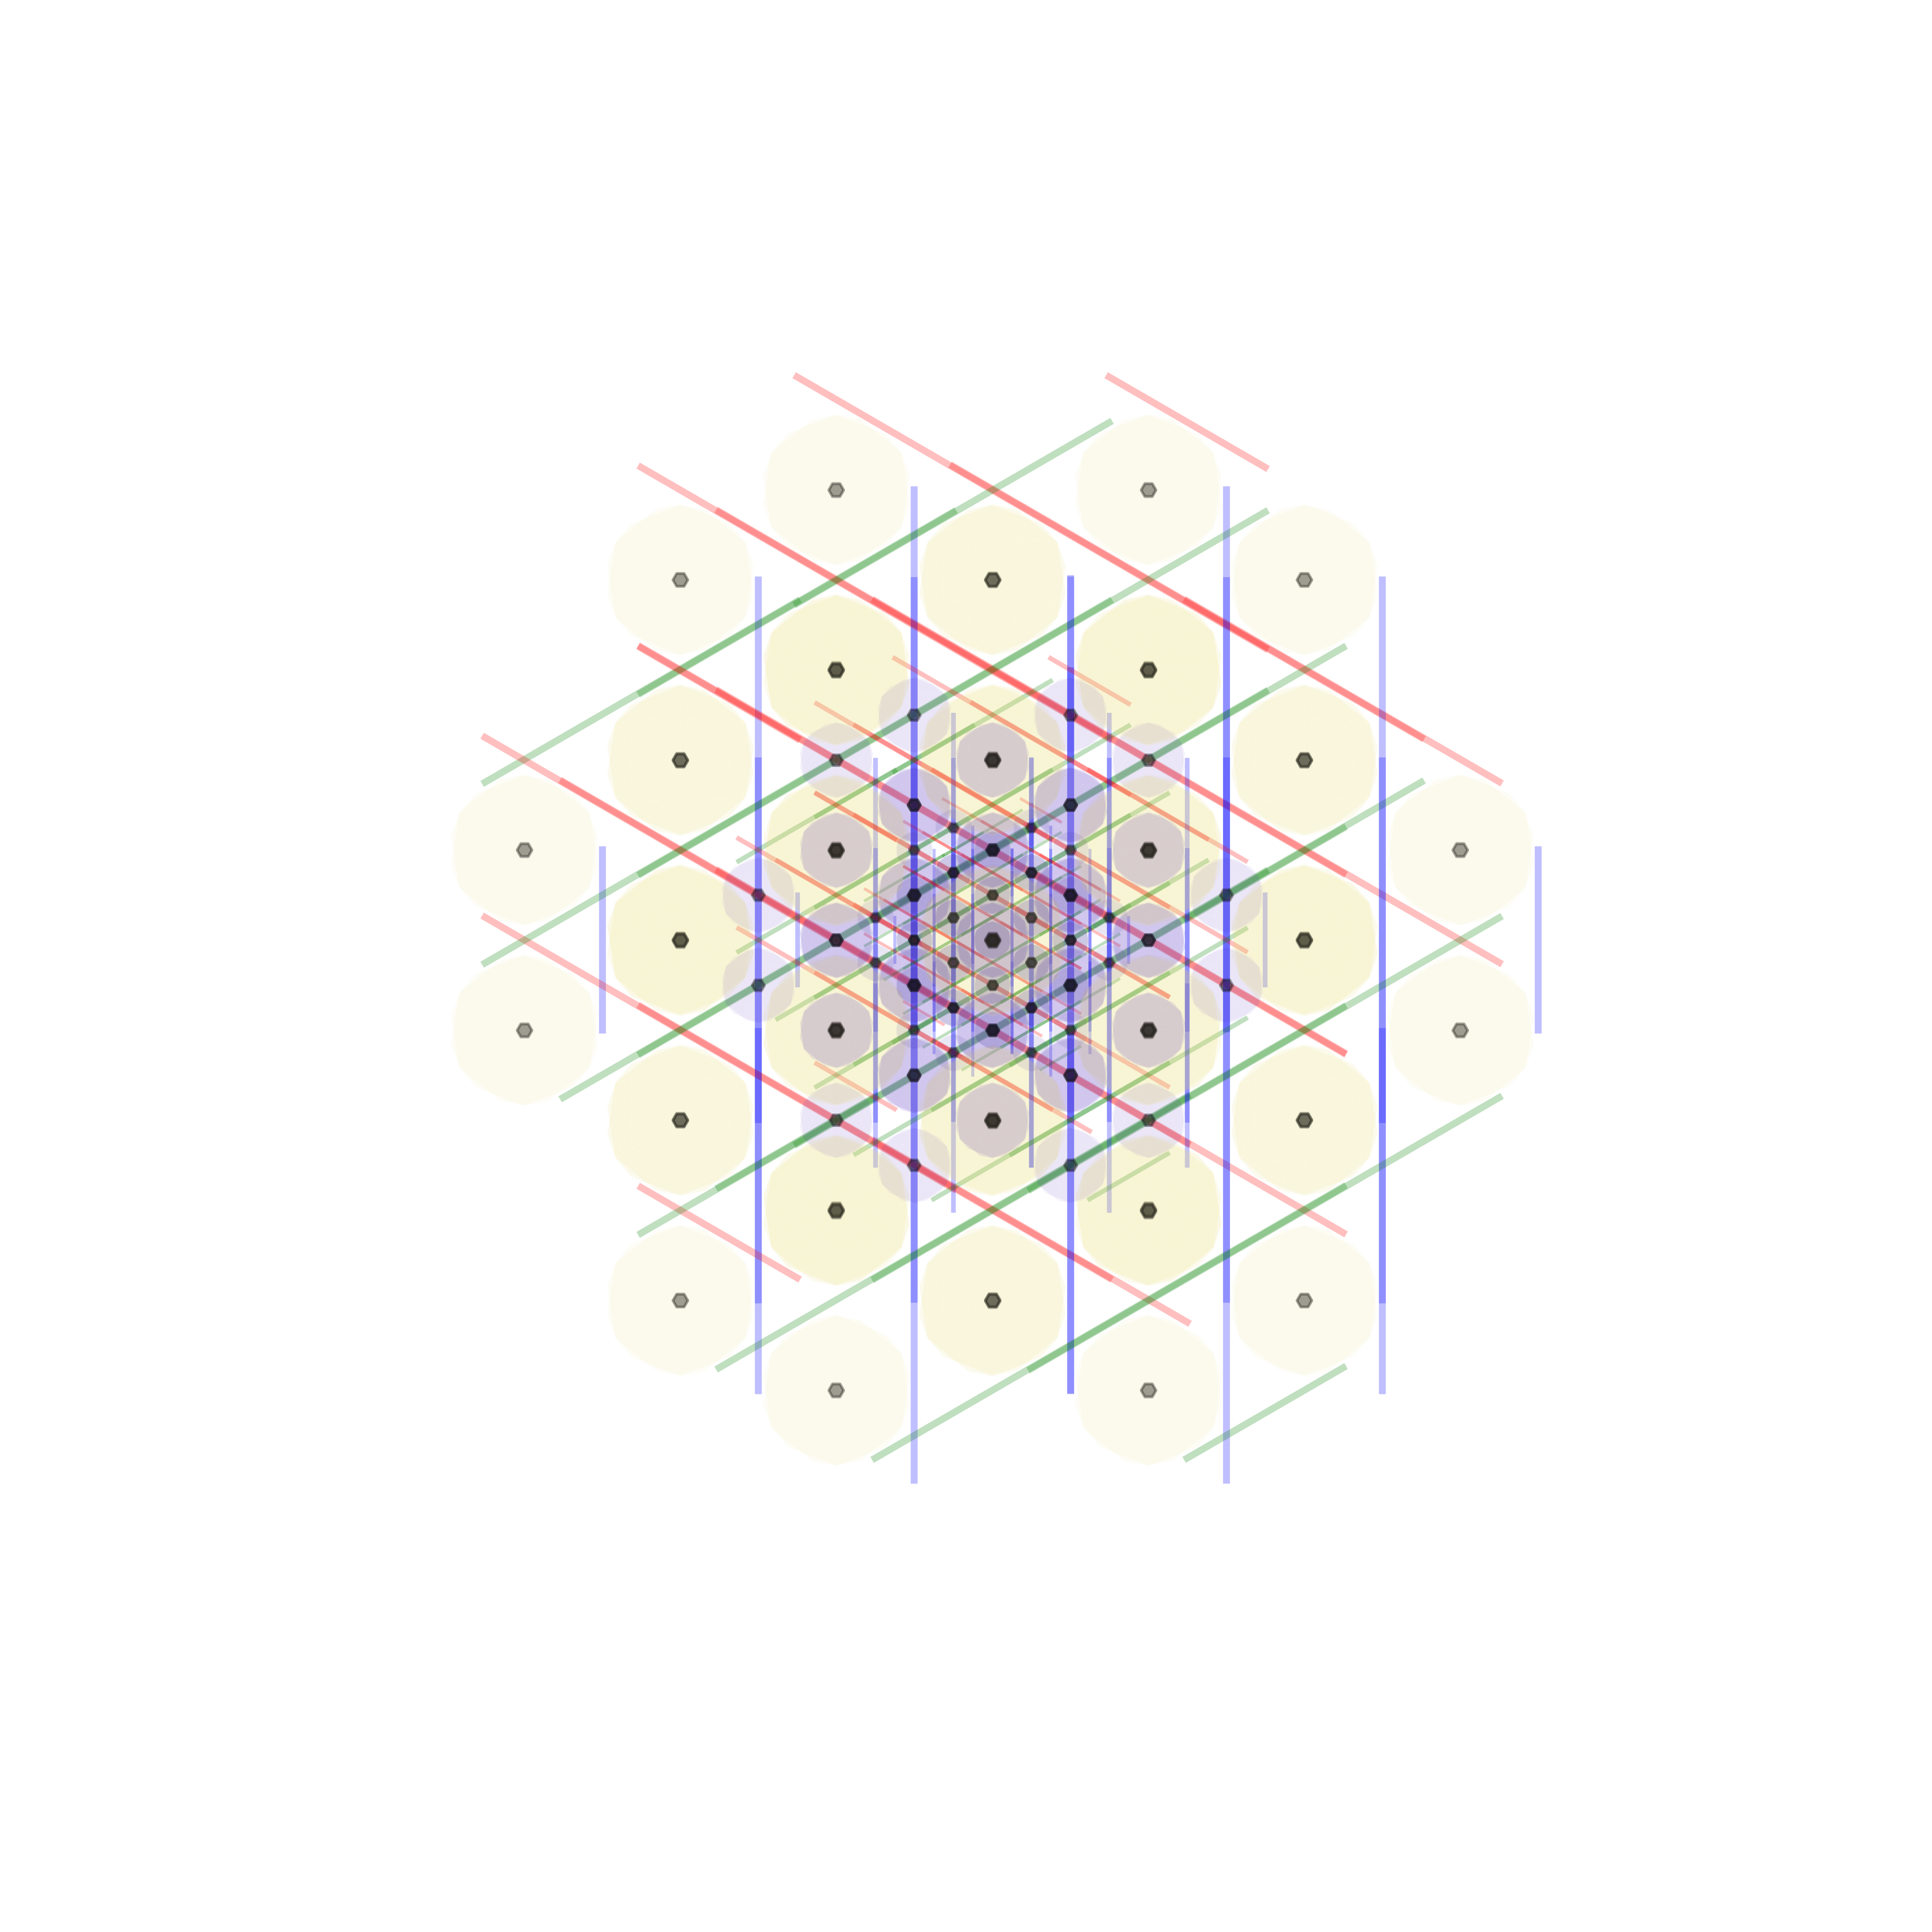
\includegraphics[trim=150 150 150 155,scale=.75]{intro} \caption{Illustration of \AAAB{} at three
different scales. \label{fig-intro}} \end{figure}


\section{ Introduction to Floats and Spatial Partitioning with \AAAB
}\label{introduction-to-floats-and-spatial-partitioning-with-a15}

Binary floating-point numbers, commonly known as \emph{floats}, are notorious for giving slightly different, \emph{approximately
correct} answers.

\[ \dfrac{\mathit{\scriptstyle significand}}{2^{\mathit{exponent}}} \]

Akin to the expression above\footnote{Exponents are effectively signed---\emph{bias} is an implementation detail---and $2^{-n}$
is $^1/_{2^n}$.}, floats resemble fractions or ratios. Their integer numerators cycle linearly $0$--$\mathit{significand}$ once
per denominator, whereas their log-linear denominators must double or split on strict powers-of-two. This representation
approximates the vast majority of rational, base$_{10}$ numbers, and accumulating tiny, order-dependent rounding errors is
\emph{expected}. There are ninety-three approximations in the first one-hundred $^1/_n$ reciprocals alone, where denominators are
\emph{most} dense.

Floats shed the stability of integers to dramatically boost their reach. Hardware-accelerated for decades in pursuit of ever-more
floating-point operations per second (FLOPS), a~single, fixed-bit memory format meaningfully ranges from quantum foam to cosmic
web. Floats are \emph{inescapably} abundant---the sand of software---their skillful workings endow modern data structures with
great strength and timeless clarity.

This research accepts and embraces binary floats as they are. It scales both the \AAAB{} phase structure, also known as
$\beta$--$W$, and its corresponding Voronoi honeycomb, \tWPh, to align with precise, IEEE 754-2008 floating-point specifications.
Each honeycomb cell collapses its internal, 3D floating-point coordinates to an integer-encoded \AAAB{} site at its core, and
together, cores identify a~compact, higher-order space---a~well-rounded snapshot of the original, 3D floating-point space---where
every high-dimensional \AAAB-encoded coordinate mirrors an exact 3D float.

This research applies to IEEE 754-2008 base$_{2}$ floating-point numbers of all bit sizes, and may refer to them as
\emph{binary$_{64}$}, \emph{binary$_{32}$}, \emph{base$_{2}$ floats}, or simply \emph{floats}. For coding and analysis purposes,
binary$_{64}$ is preferred, due to its large size and prevalence in modern CPUs. For baselines and performance comparisons,
binary$_{32}$ is preferred, due to its widespread presence in hardware, software, and network stacks.

The nomenclature and parlance used throughout is primarily that of crystallography, borrowing from other disciplines as
necessary.

\begin{figure}[!ht]\capstart 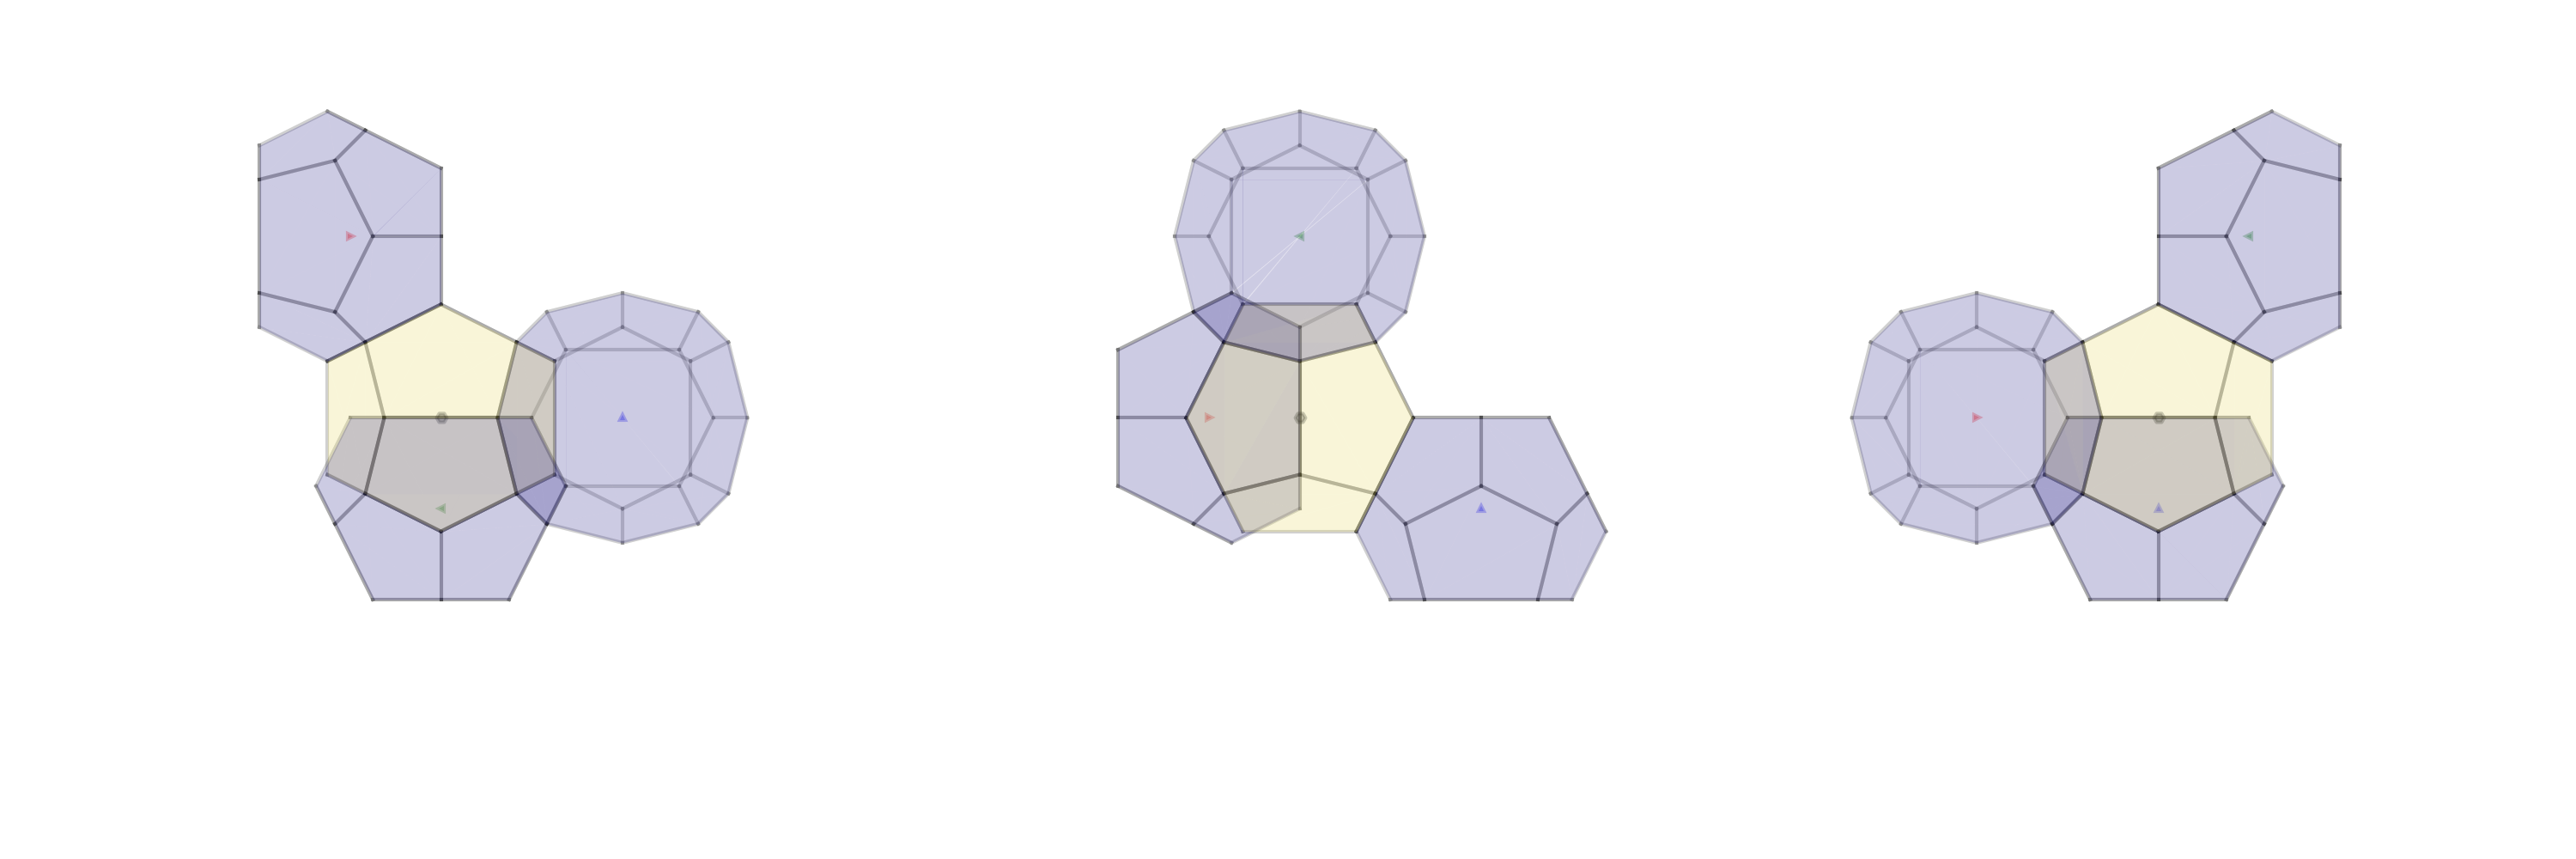
\includegraphics[trim=25 50 25 0,scale=.55]{cell2} \caption{Left-handed $^1/_2$ unit cell.}
\label{fig-cell2} \end{figure}

\subsection{ Foundational Understanding of \AAAB{} and Spatial Partitioning
}\label{foundational-understanding-of-a15-and-spatial-partitioning}

Partitioning virtual spaces is a~matter of fairness. ``Fairness," as it applies to transformations on structures in 3D space, is
a~measure of isometry and isotropy---reducing the bit space \emph{must not} significantly warp distances and angles between any
two sites. While isometry on its own is readily achievable, combining it with isotropy is much more difficult. The $SO(3)$ group,
or the set of all possible 3D rotations, is spherical---highly-isotropic structures appear ``rounder" from the perspective of an
individual site---and simply cannot fit nicely inside a~cubical lattice ``box". This innate tension between
translation-preserving symmetries and rotation-preserving symmetries drastically shrinks the pool of N-fold designs available to
perfectly isometric 3D lattices. In accordance with the crystallographic restriction theorem, C12 is the maximum coordination
number, and the only possible angles are 180$^{\circ}$ (2-fold), 120$^{\circ}$ (3-fold), 90$^{\circ}$ (4-fold), and 60$^{\circ}$
(6-fold)---icosahedral designs (5-fold) with $I_h$ symmetry are not possible.

\AAAB{} eschews perfect isometry. It trades 100\% identical sites for a~blended mix of exactly 75\% C14 major
sites---axes-aligned tetradecahedral layers (\WP) or cubes (\TS) with 14 connections each---25\% C12 minor sites---pyritohedral
voids (\WP) or cubes (\TS) with 12 connections each---and two different site-to-site distance metrics. True 5-fold symmetry
appears in the form of alternating left- and right-handed sites with $T_h$ \emph{pyritohedral} symmetry, an isometric subgroup
(4-of-10 3-fold axes) of the full icosahedral symmetry group $I_h$. This localized asymmetry drastically increases isotropy (13.5
mean coordination) without impacting long-range isometric order.

\begin{figure}[!ht]\capstart 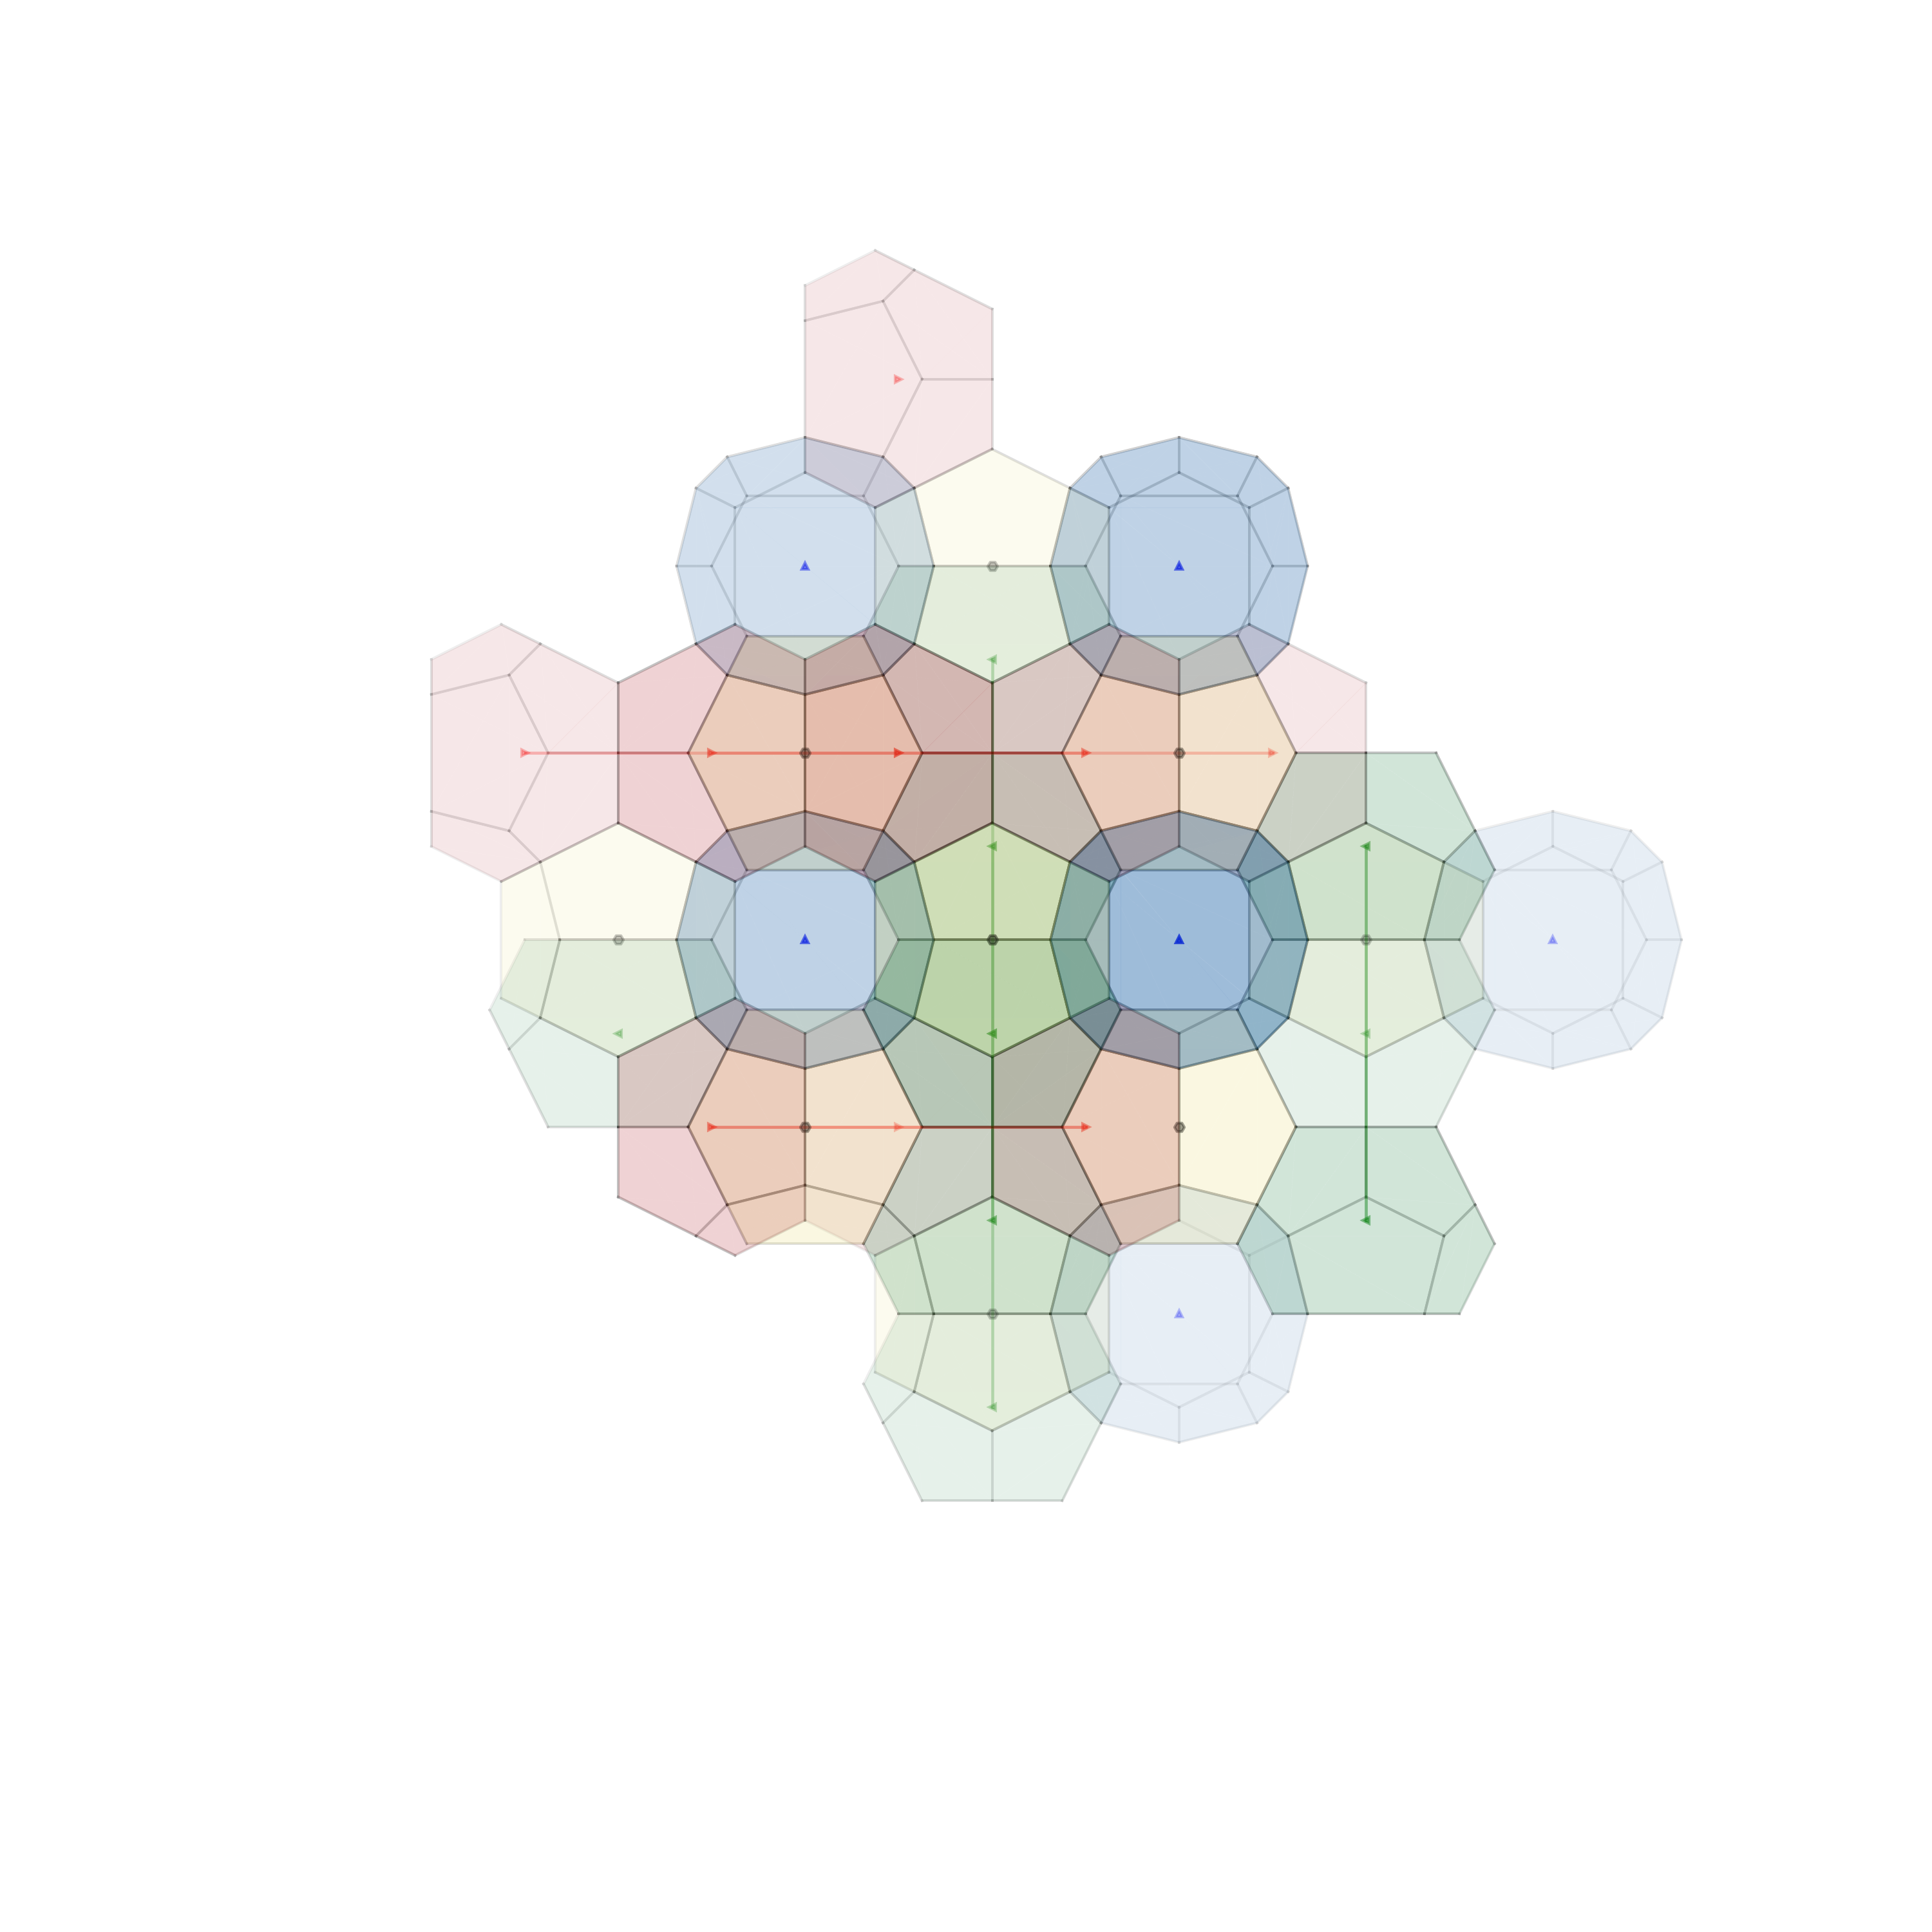
\includegraphics[trim=130 140 80 50,scale=.35]{wp}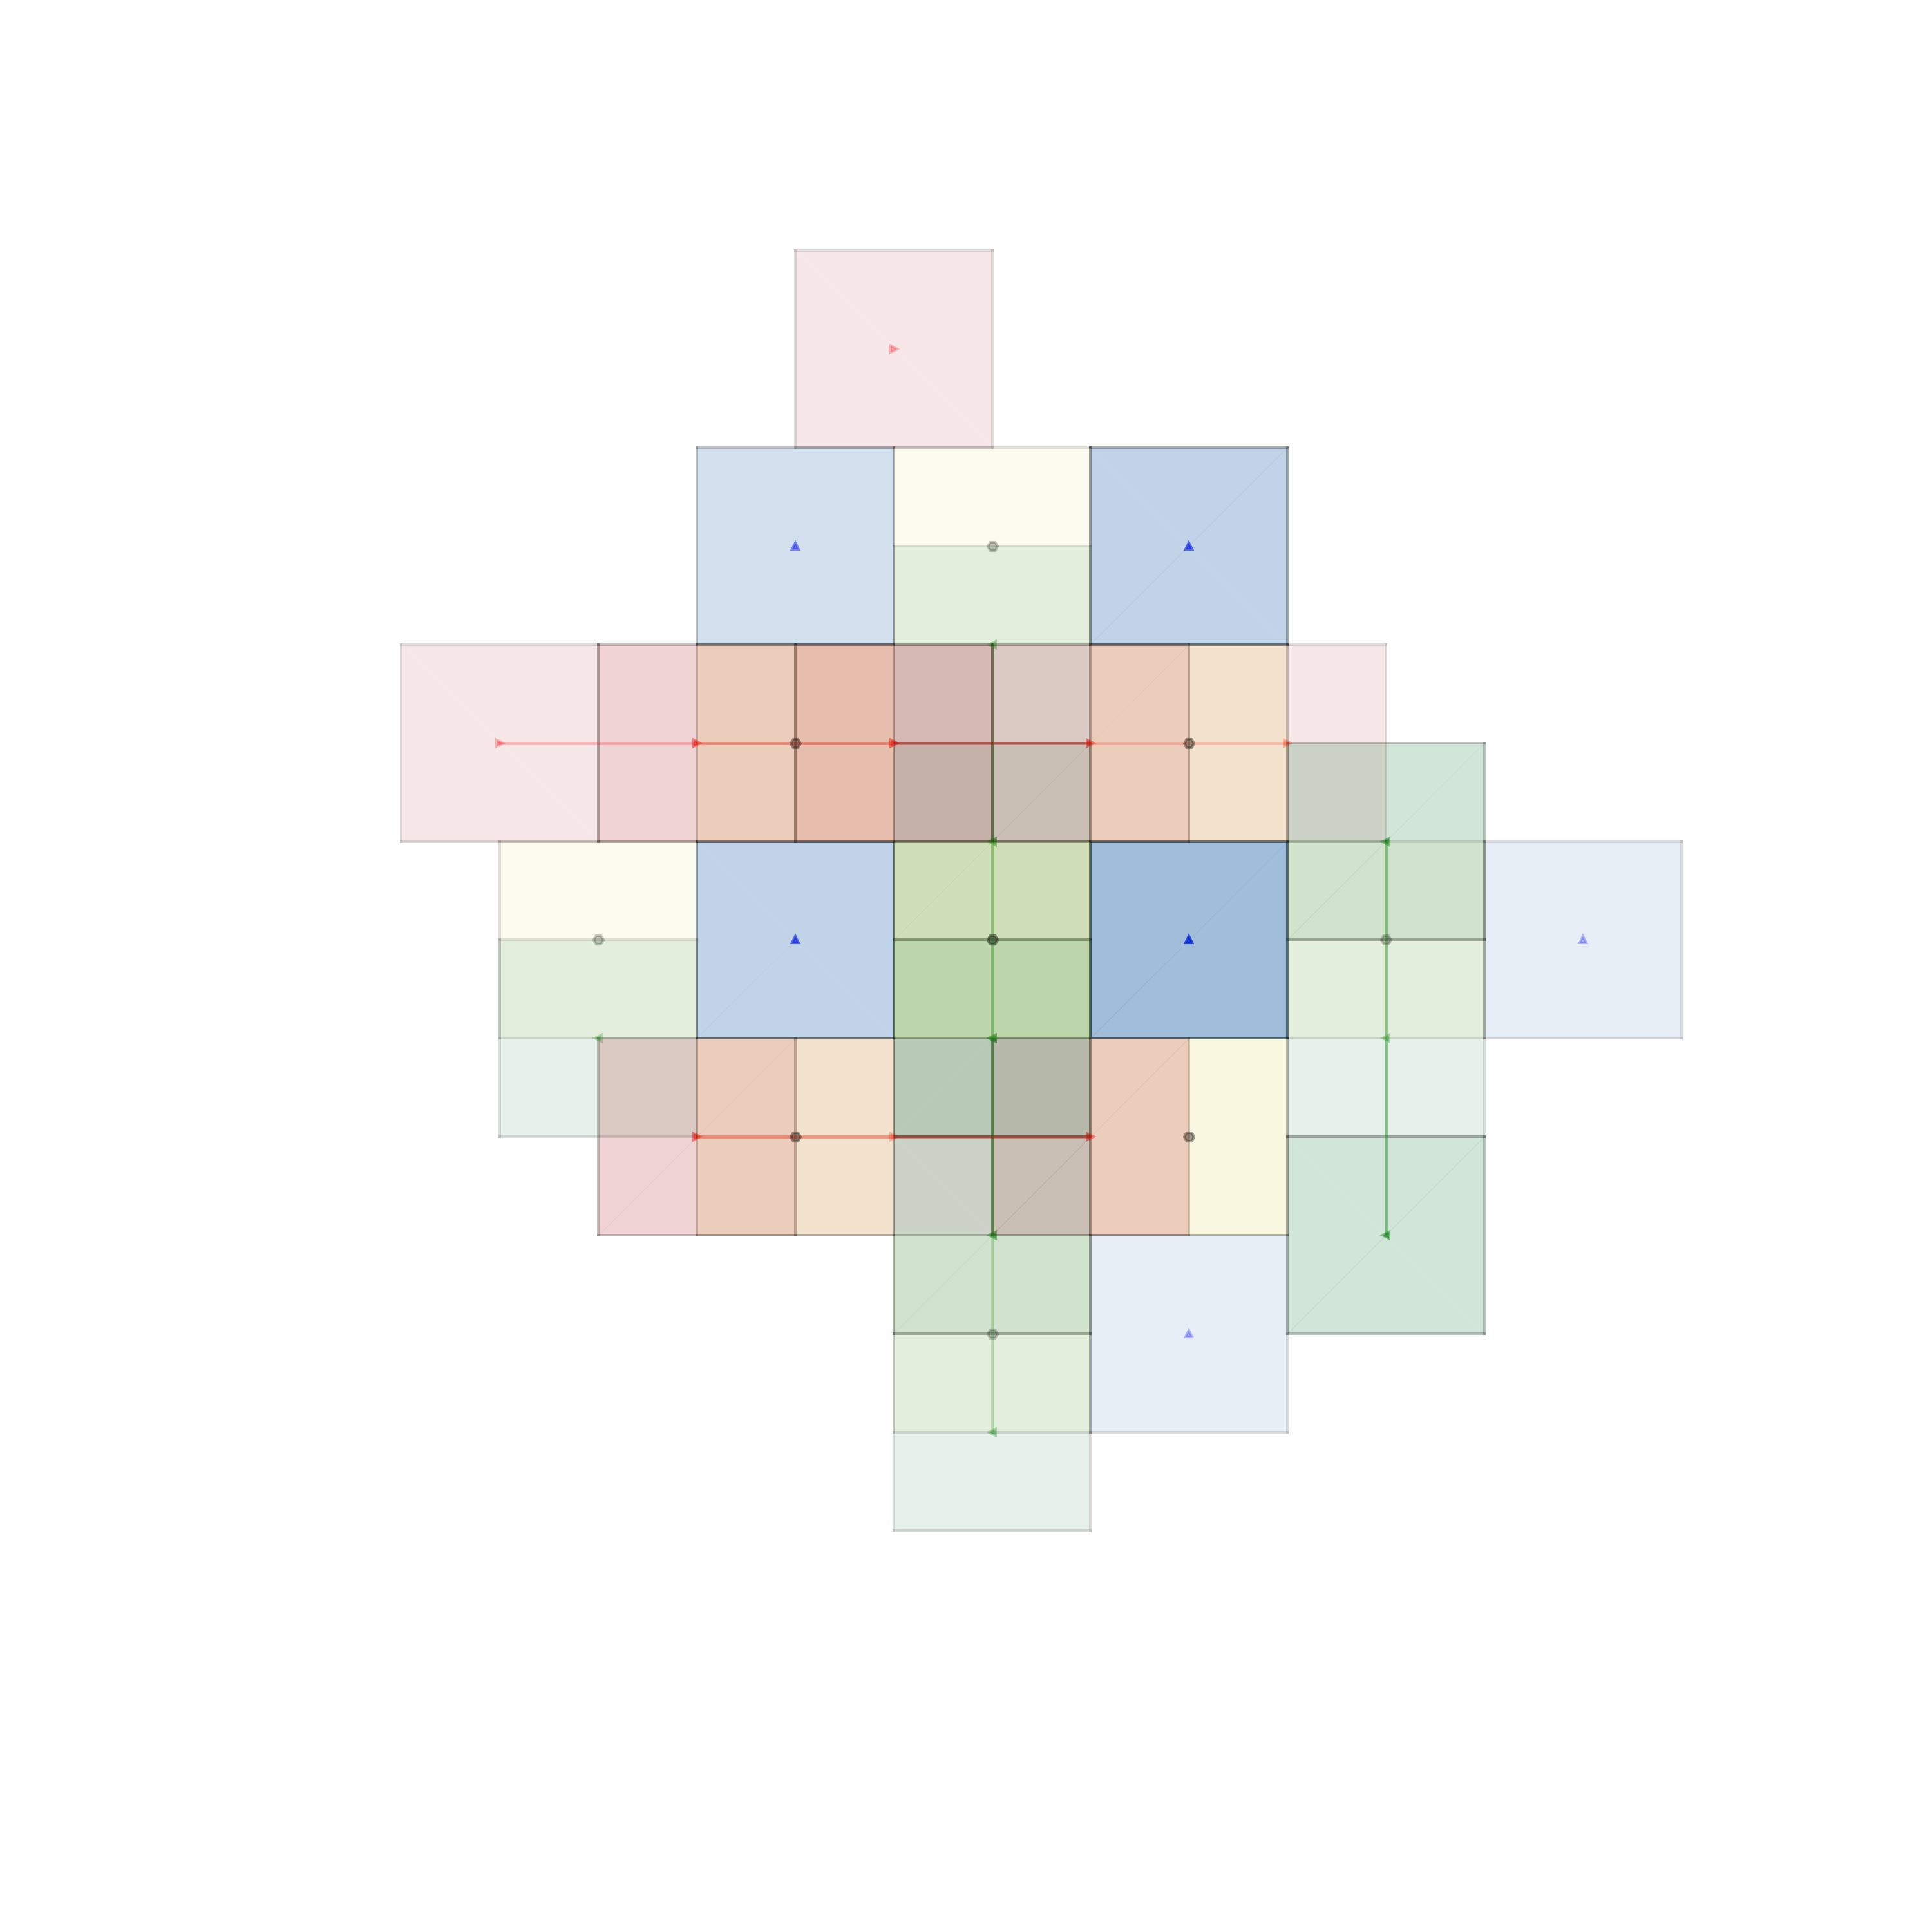
\includegraphics[trim=130 140 80 50,scale=.35]{ts}
\caption{\TWPh{} (left) and \tTSp{} (right). \label{fig-wp} \label{fig-ts}} \end{figure}

In a~sense, \AAAB{} is already binary. Its fractional lattice coefficients use nothing but the first three multiples of $2^{-2}$,
and all eight basis sites are perfect binary floats. Quadruple its fractional coordinates into the integers, and its two,
site-to-site distance metrics become $2$ (major-major) and $\sqrt{5}$ (major-minor). $\sqrt{5}$ is the hypotenuse of a~2:1 right
triangle and the crux of the golden ratio. \AAAB{} can be defined at unit scale without stability issues. However, at any scale,
\AAAB{} only represents the destination encoding, leaving open the question of \emph{how} higher-density bit spaces should
discretize themselves to a~valid \AAAB{} site. In other words, finding the nearest site requires a precise definition of
\emph{nearest}.

The first definition, depicted in \autoref{fig-wp} (left), is available to any 3D point set. Starting from an \AAAB{} integer
crystal lattice, identify its Voronoi honeycomb from the set of inflection points between neighboring \AAAB{} sites---edges in
this secondary structure have exactly two nearest neighbors in \AAAB{}, and vertices have three or more---and \tWPh{} appears.
A~simpler, less isotropic definition of \emph{nearest} is also available to \AAAB{}. As seen in \autoref{fig-ts} (right), when
the angle between sites in the secondary structure is fixed to 90°---forcing exactly six nearest neighbors and filling the space
with \emph{unit} cubes---\tTSp{} emerges instead. The price for this simplicity is reduced spatial accuracy and more directional
aliasing.

\subsection{ Spatial Indexing and Related Spatial Partitioning Methods
}\label{spatial-indexing-and-related-spatial-partitioning-methods}

Spatial partitioning is closely associated with spatial indexing. In this context, the partitioner is more dynamic and
specific---space is split on maximally-coincident hyperplanes, or enclosed within minimally-overlapping polytopes, for the
purposes of cataloging sites and facilitating retrieval. Incoming sites are unlikely to adhere to any meaningful symmetry and
freely utilize the full range and precision of the ambient space. This ignorance of an implied external structure is critical for
spatial indexing, but renders well-known binary space partitioners (BSP), like octrees and KD trees, and bounded-polytope
solutions, like R-trees, R$^*$-trees, and its derivatives, less attractive as \emph{implicit}, memory-efficient, interactive
virtual space partitioners, because their preferred hyperplanes and polytopes do not maintain the spatial symmetries of the
ambient space. However, if they did maintain ambient symmetries, the resultant structures might resemble objects that are
comparable to \AAAB{}: space groups and space-filling honeycombs.

\subsection{ Comparative Analysis of \AAAB{} with Space Groups and Honeycombs
}\label{comparative-analysis-of-a15-space-groups-and-honeycombs}

Three-dimensional space admits fourteen crystallographic lattice types known as Bravais lattices---fourteen distinct,
prototypical pairings between one-of-seven lattice systems and one-to-four lattice centerings---and every discrete,
\emph{periodic} tesselation of 3D space shares its translational isometries with a~Bravais lattice. Non-translational isometries,
such as reflections and rotoinversions, are known as 3D point groups, and the thirty-two that satisfy the crystallographic
restriction theorem are deemed the crystallographic point groups. The complete set of 230 space groups emerges from all
isomorphic combinations of the fourteen lattice types with the thirty-two crystallographic point groups, and fully characterizes
any periodic tesselation of 3D space.

\begin{figure}[!ht]\textbf{(todo) Table.} $Pm\bar{3}n$ (223) alongside other groups.\end{figure}

\AAAB{}'s space group, $Pm\bar{3}n$, pairs the $O_h$ symmetry of the $cP$ Bravais lattice with the $T_h$ pyritohedral symmetry of
the $m\bar{3}$ crystallographic point group. $T_h$ pyritohedral symmetry is an isometric subgroup of the
\emph{non-crystallographic}, full icosahedral symmetry group, $I_h$. Crystallographic point groups with $T_h$, $O$, and $T_d$
symmetries are all order 24, and second only to order 48, $O_h$ cubic symmetry. Since $T_h$ is the maximal subgroup between $O_h$
and $I_h$---between the existing cubical-octahedral isometries of \AAAB{}'s Bravais lattice and the highly-desirable,
\emph{non-crystallographic} icosahedral isometries of $I_h$---any point group with higher order than $m\bar{3}$ is also more
cubical. The link from $m\bar{3}$ to $I_h$ symmetry through $T_h$ symmetry is strong evidence that $m\bar{3}$ is isotropically
ideal.

\begin{figure}[!ht]\textbf{(todo) Table.} \AAAB{} alongside other honeycombs (mean coordination, etc).\end{figure}

\begin{description}

  \item[(todo) Tetrahedral-octahedral honeycomb] Simplectic, quasiregular honeycomb and face-centered cubic (FCC or $A_3$ or
    $D_3$) lattice; mean coordination 12; space group $Fm\bar{3}m$ (225); vertex- and edge-transitive; ideal 3-space packing of
    identical spheres; reciprocal lattice is BCC.

  \item[(todo) Tetragonal disphenoid honeycomb] Uniform honeycomb and body-centered cubic (BCC or $A_3^*$ or $D_3^*$) lattice;
    mean coordination 8; space group $Im\bar{3}m$ (229); vertex-, face-, and cell-transitive; reciprocal lattice is FCC; ideal
    k-space samples in $R^3$.

  \item[(todo) Rhombic dodecahedral honeycomb] Non-uniform Voronoi honeycomb of FCC lattice; mean coordination 5.5; space group
    $Fm\bar{3}m$ (225); edge-, face-, and cell-transitive; 3-space parallelohedron.

  \item[(todo) Bitruncated cubic honeycomb] Uniform Voronoi honeycomb of BCC lattice; mean coordination 4; space group
    $Im\bar{3}m$ (229); vertex-, edge-, and face-transitive; 3-space permutohedron; best-known ideal foam (Kelvin problem) for a
    century, then superseded by \tWPh{}.

\end{description}


\section{ Experimental Design, Implementation, and Validation }\label{experimental-design-implementation-and-validation}

\textbf{(todo)} State reasoning for finding the smallest-possible integer representation, if any; show unstable configuration;
walk through construction of \AAAB{} and surrounding it with \tWPh, identifying its minimum prescale factor along the way; relate
integer scaling to fraction-like floating-point definition from introduction; add the next layer of lattice and additional
prescale due to separation distance; binary splits of this final prescale are ``binary" scales, multiples of these splits are
``stable" scales, and everything else is ``unstable"; bits shuffle cleanly between range and density, facilitating the definition
of subspaces; show \TS{} at \WP's prescale and frame volume difference as an error domain.

\newpage{} % TODO: Remove when section above is complete.

\subsection{ \AAAB.py's Experimental Design and Exploration }\label{a15s-experimental-design-and-exploration}

\textbf{(todo)} Explain \AAAB.py generation process, reasoning, capabilities, and assertions; describe main image and such things
as $N_1$ (cell width), $\epsilon_N$, $\epsilon_\delta$, $\epsilon_\Delta$, and $\epsilon$.

\begin{figure}[!hb] 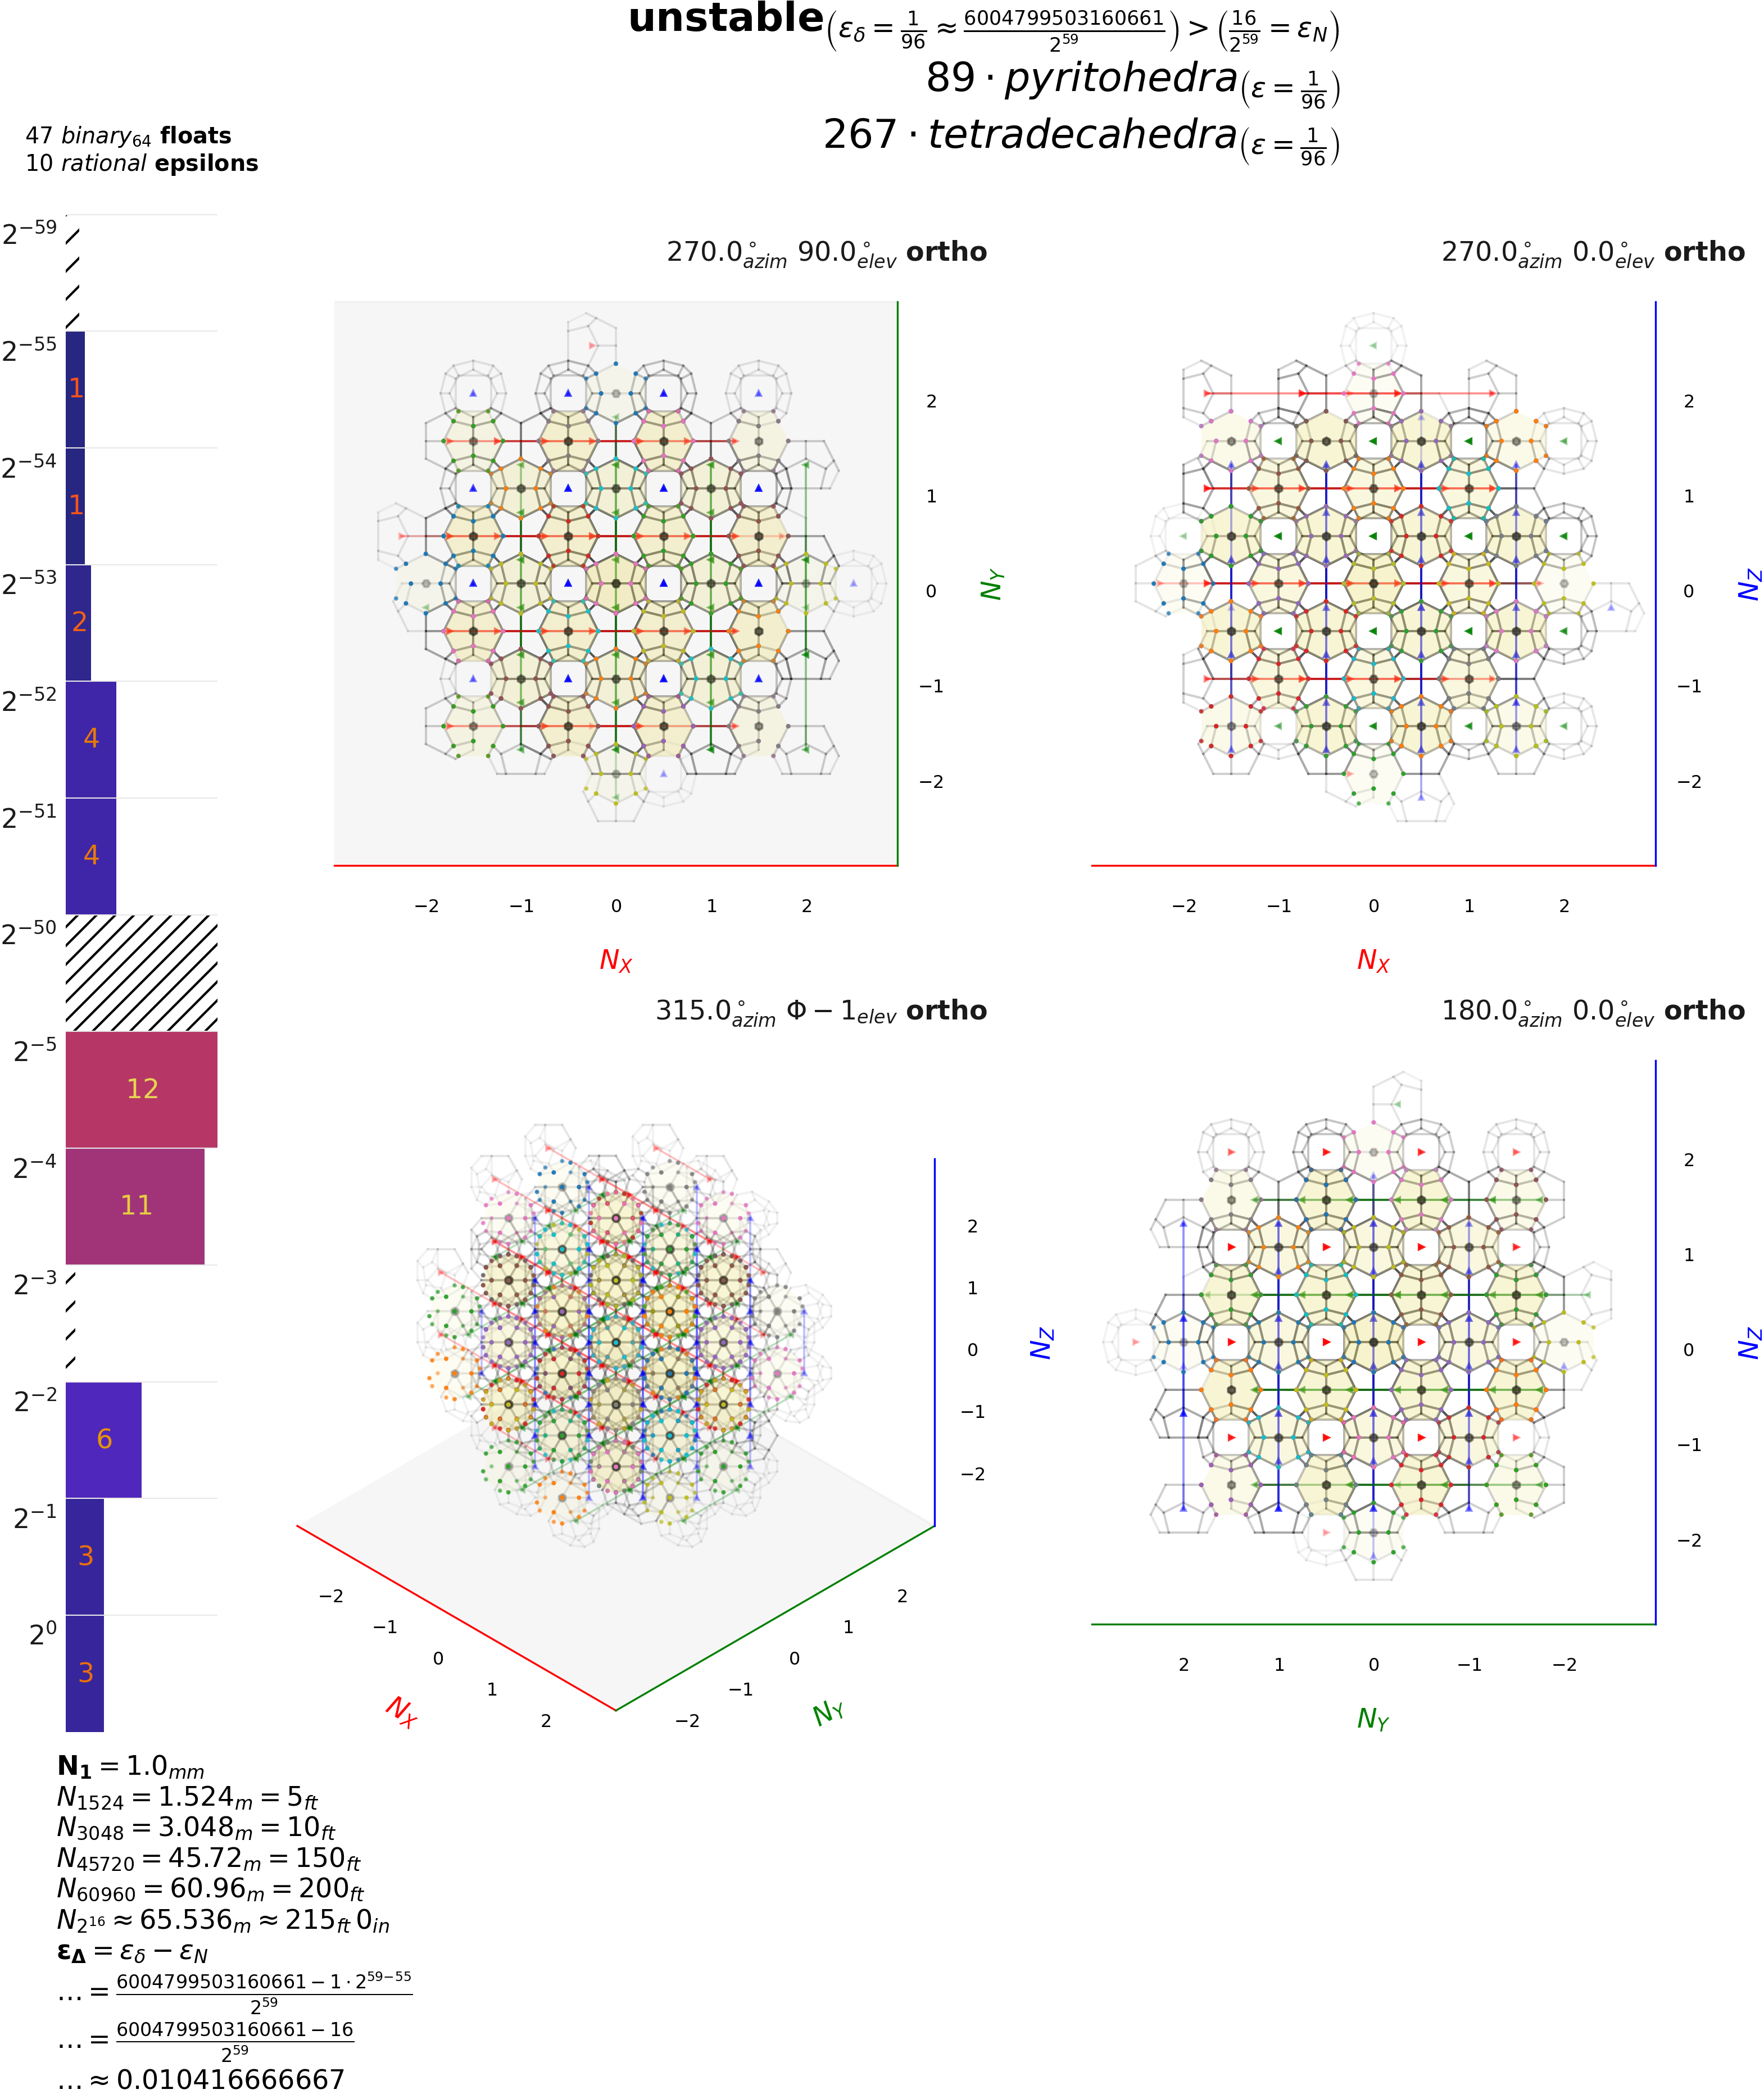
\includegraphics[scale=.5]{main} \label{fig-main} \end{figure}

\subsection{ Validation Techniques and Statistical Analysis }\label{validation-techniques-and-statistical-analysis}

\begin{figure}[!hb] 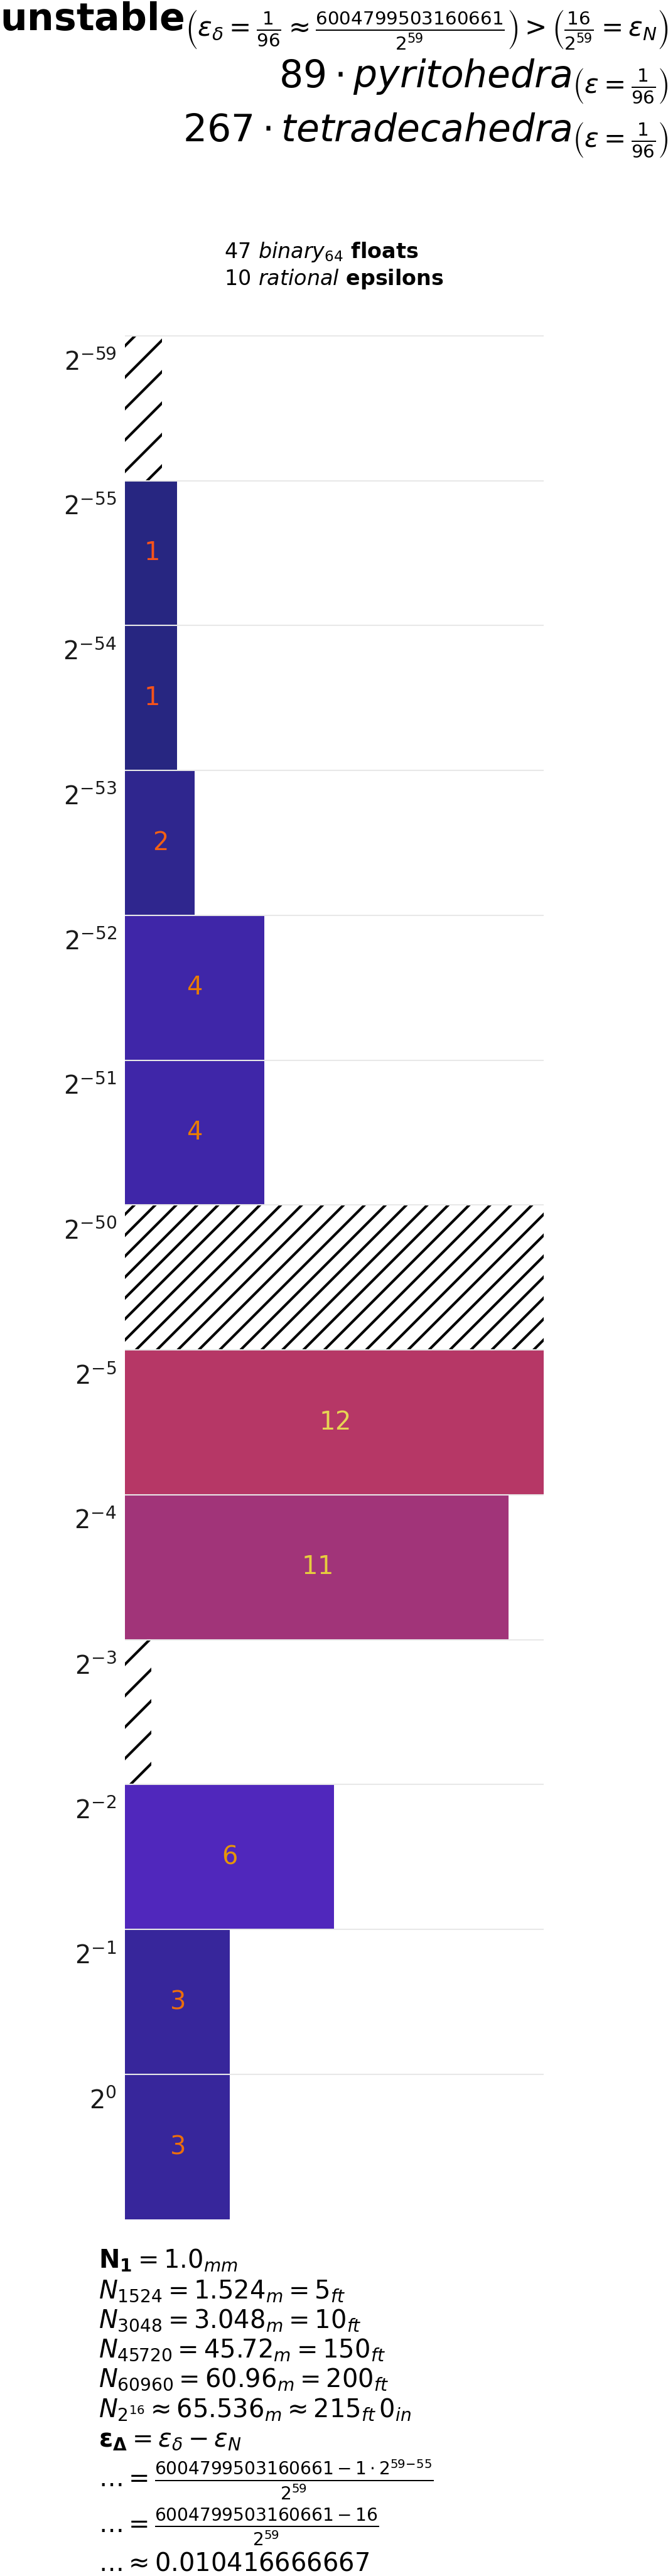
\includegraphics[width=.325\textwidth]{histu} 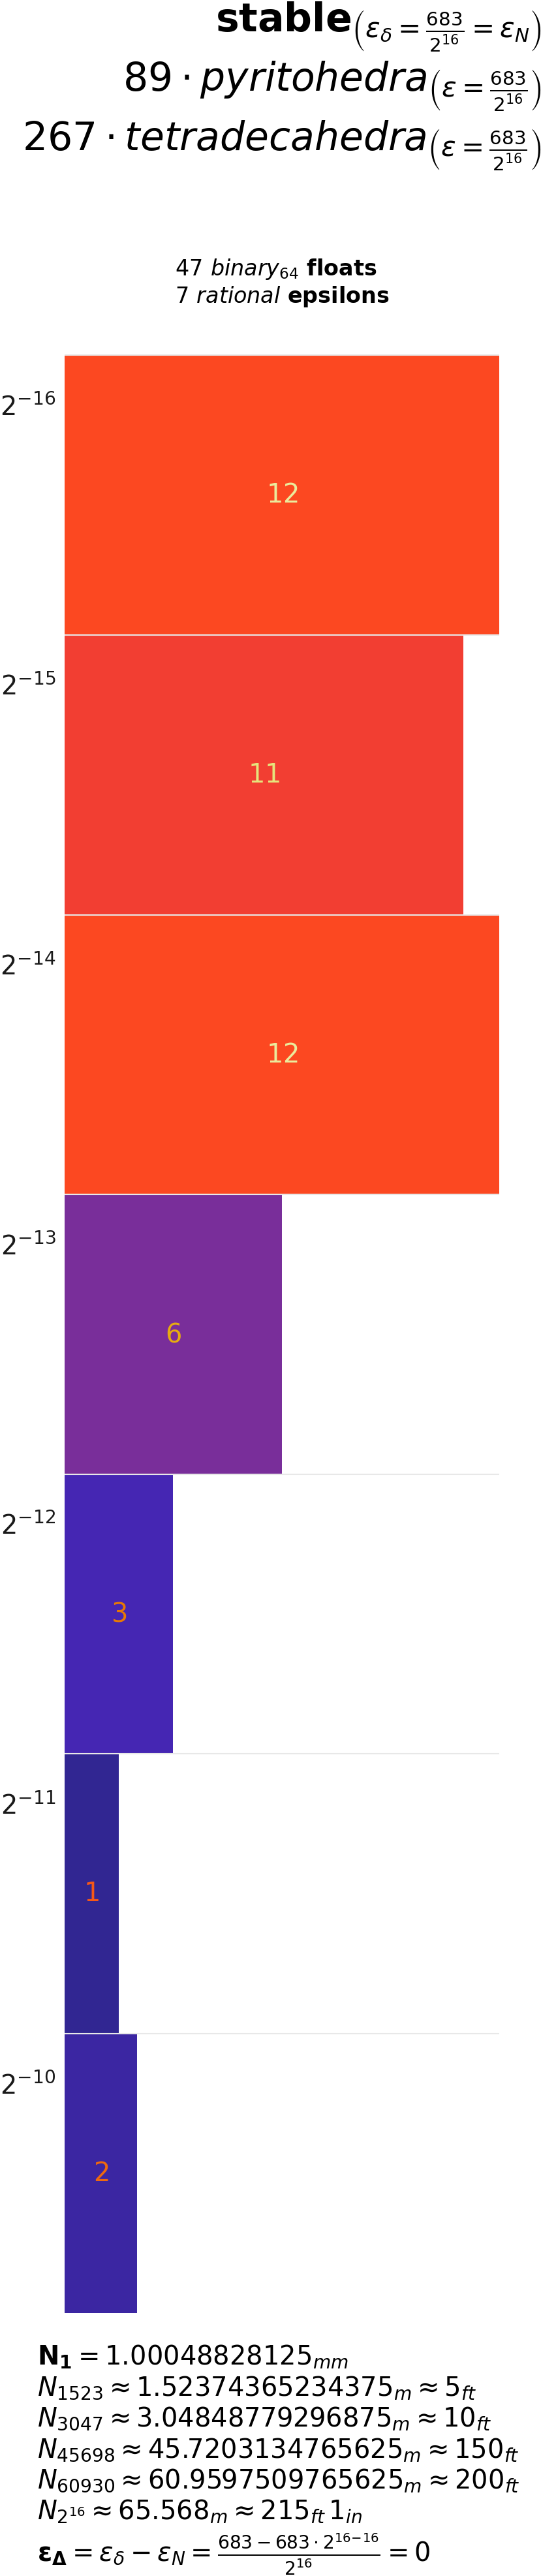
\includegraphics[width=.265\textwidth]{hists}
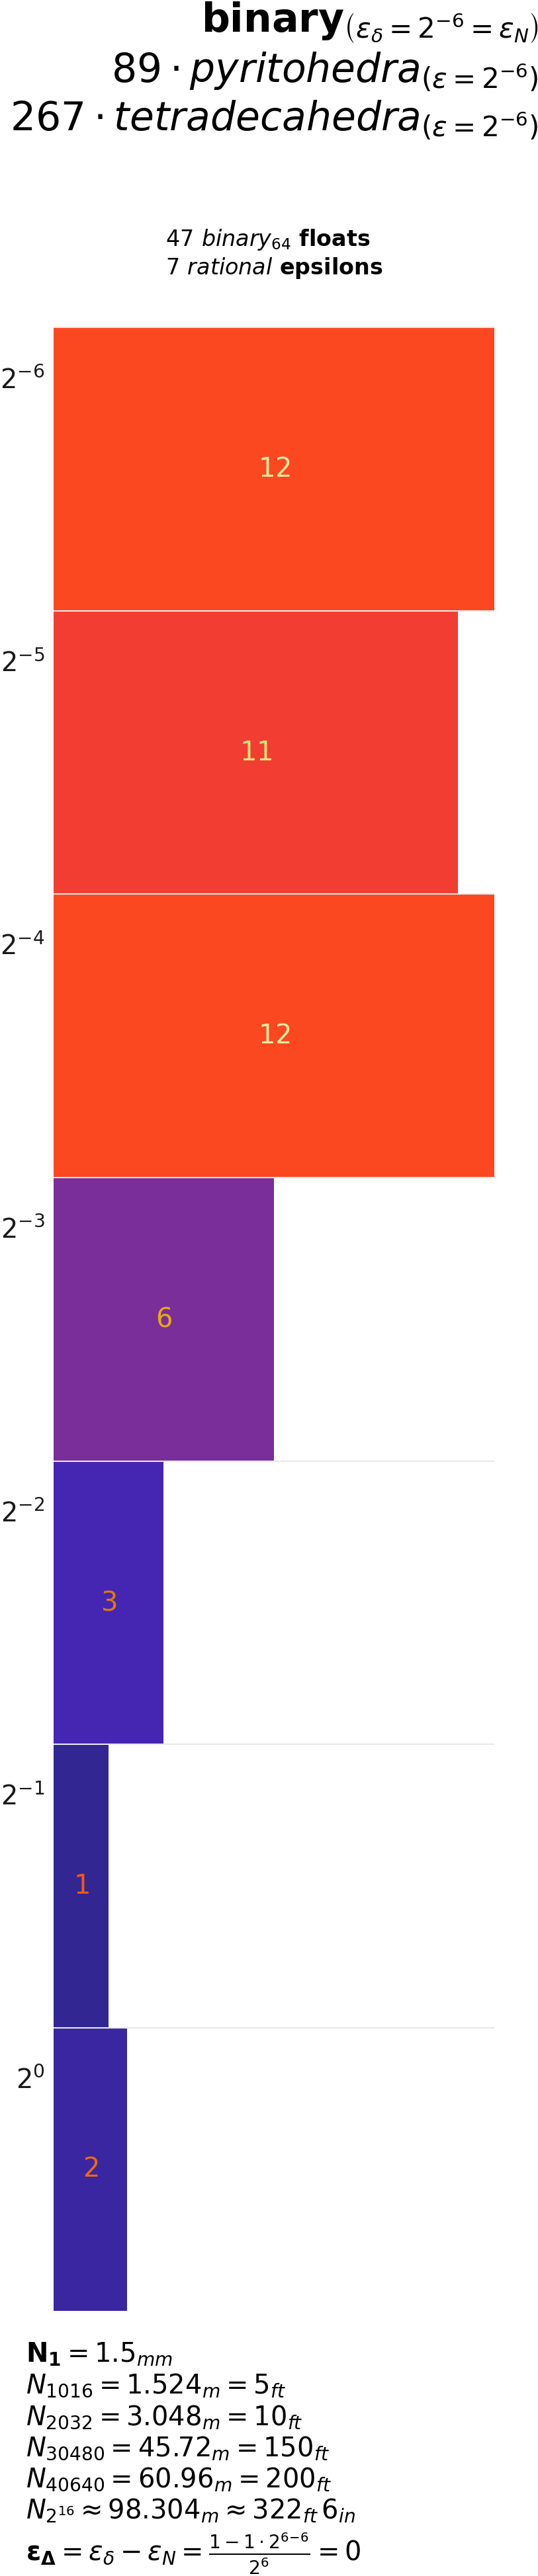
\includegraphics[width=.26\textwidth]{histb} \caption{ Example \emph{unstable} (left) \label{fig-histu}, \emph{stable}
(middle) \label{fig-hists}, and \emph{binary} (right) \label{fig-histb} configurations. } \end{figure}

\textbf{(todo)} Explain \AAAB.py histogram bar graph and its epsilons; show unstable configurations generating a~smattering of
epsilons and unused gaps; contrast this with gapless, sequential configurations that always generate a~limited number of epsilons
(stable) or an exact number (binary).


\section{ Results Interpretation, Insights, and Limitations }\label{results-interpretation-insights-and-limitations}

\AAAB{} has a~long and storied history, from holding the high-temperature superconductor record for decades, to its close
association with other interesting structures---such as \tWPh{} and \tTSp---each with their own unique qualities. \TWPh, in its
relaxed, non-polyhedral ``bubble" form (combinatorially equivalent to the polyhedral honeycomb), consistently yields
highly-isotropic measurements from different physical quantities, including thermal expansion rate, compressional load transfer,
photonic wave propagation, and quantum noise distribution. \AAAB's position is further reinforced through its crystallographic
space group properties, such as an exceptionally high coordination number (mean of 13.5 connections per site), second-highest
symmetry order (24), and maximal intersection with the \emph{non-crystallographic} $I_h$ group. Centered on \tWPh---the
best-known equal-volume partitioner of 3D space and lowest-energy solution to the Kelvin problem---and simultaneously compatible
with \tTSp---an attractive alternative to \WP-based discretization when trading spatial inaccuracy for performance is acceptable
or desirable---makes \AAAB{} uniquely qualified for partitioning interactive 3D space.

\subsection{ Interpretation of Findings and In-Depth Insights }\label{interpretation-of-findings-and-in-depth-insights}

This research presents \AAAB{} as the ideal, coordinated partitioner of shared, interactive virtual space. It highlights \AAAB's
innate mapping to hardware floating-point representations, and its compatibility with global measurement systems. It details two,
high-dimensional addressing schemes, and explains their differences in terms of lattice centering, chiral balancing, and
interlocking extrema. \AAAB's numeric floating-point stability is confirmed, and three distinct classifications---\emph{binary},
\emph{stable}, and \emph{unstable}---are identified. It asserts the binary floating-point stability of \tWPh, \tTSp, and \AAAB{}
itself, using both a~series of mathematical statements and generated empirical evidence. It constructs well-defined,
heterogeneous environments, and characterizes how additional bits either double the range or double the density. Original code is
shared in full, alongside detailed examples and documentation. This outcome, combined with \AAAB's body of existing materials
research, makes \AAAB{} an excellent candidate for \emph{reshaping} the metaverse.

\subsection{ Noteworthy Limitations and Topics of Concern }\label{noteworthy-limitations-and-topics-of-concern}

Regardless of addressing scheme, most on-lattice symmetry operations require follow-up translations to maintain \AAAB's desirable
invariants. \AAAB{}'s primitive unit cell contains eight valid sites---known as its basis, or crystal motif---but only one is
also a valid lattice point.

\AAAB{} is a linear space partitioner. Creating massive, open-world virtual environments is less straightforward because \AAAB{}
spaces are small, irregularly sized, and end abruptly. Federating virtual real estate in a~fifty-story skyscraper might require
independent \AAAB{} spaces per floor, or per delegable unit. This matches expectations after reclaiming unused dynamic
floating-point range as memory savings, but fast-paced transitions at spatial joins are potential sources of bugs, complexity,
and overhead.

This research generates \AAAB{} crystal-lattice cuboids with rectangular faces, and with edge lengths in proportion to each
dimension's allocation of the total bit space. Cuboids best-encode spaces like playing fields and office buildings---spaces with
high average utilization, and clear, axes-aligned boundaries---and are less efficient for spaces with arbitrary terrain,
irregular boundaries, or internal holes. Such features generate effectively unreachable pockets of addressable space. However,
compared to the unused dynamic range of floats, this underutilization is much simpler to quantify.

Cited \WP{} research uses a~relaxed form of \tWPh{} to satisfy Plateau's laws and the constraints of the Kelvin problem. This
structure is combinatorially equivalent to the polyhedral form, albeit with softer angles and perfectly equal-volume pyritohedra
and tetradecahedra. Results from these studies may not transfer cleanly. However, discrepancies are limited to \WP-based
discretization claims and not \AAAB{} itself.

This research facilitates the long-term storage and analysis of human-generated spatial tracking data---personally identifiable
information (PII) with both legal and ethical requirements---and \emph{demands} that implementers honor and regard it with the
utmost care and respect.


\section{ Immediate Potential and Future Prospects }\label{immediate-potential-and-future-prospects}

\subsection{ Universal Compatibility and Widespread Applicability }\label{universal-compatibility-and-widespread-applicability}

\textbf{(todo)} L/R balancing for both Unreal and Unity; reliably mutate, consolidate, or replay from the edge; clean mapping
into global measurement systems; spatial range limits are implicit anti-cheating mechanisms; range limiting combined with other
symmetry-reliant techniques expected to save more memory than \emph{baseline} of 50\%.

\subsection{ Future Investigations and Potential for Immersive Experience
}\label{future-investigations-and-potential-for-immersive-experience}

\textbf{(todo)} Expecting to train AI bots; expecting to capture high speed games; resultant libraries not limited to metric
spaces, could also apply to eg. function spaces; investigate rotating \AAAB{} favorably with respect to expected traversal
patterns, eg. Miller index $(111)$, and boost effective isotropy; consider ways to efficiently carve terrain, holes, and
non-planar or axes-misaligned boundaries; seek esoteric 3-space objects outside crystallography and convex geometry, eg. stars,
gyroids, quasicrystals, plesiohedra, Delone sets, and centroid network of the Laves graph; continue search for higher-dimensional
polytopes to fold and project into 3D space.


\section{ Supplementary Materials and Extended Analyses }\label{supplementary-materials-and-extended-analyses}

\subsection{ Comprehensive Code Guidelines and Replication Protocols
}\label{comprehensive-code-guidelines-and-replication-protocols}

\textbf{(todo)} Share commands to rebuild figures in this research; illuminate \AAAB.py's dark, undocumented corners; note the
binary scale's clean steppings compared to stable scaling; in some addressing schemes, the L/R orientation of major sites is
independent from that of minor sites, with four or more valid, internal orientations possible; when more than one internal
orientation is available, this research arbitrarily chooses one; all parties must know, negotiate, or discover an orientation
before transmitting coordinates; some orientations might be more favorable than others, both at the boundary and in the bulk.

\subsection{ Additional Data, Visualizations, and Mathematical Exploration
}\label{additional-data-visualizations-and-mathematical-exploration}

\textbf{(todo)} \url{https://infima.space}; A15.py itself; proofs of different assertions made, eg. 5v5 100 kbps per user
baseline; tables of vertices; list figures of interesting heterogenous environments; note how surrounding minor sites with a~7/5
pyritohedron generates correct \WP{} spacing and possible dual space; support and recommend $2^{-6}$ as the preferred default
scale; note coincidence of \AAAB{} integer scale, \TS{} unit scale, and favorable $2^{-6}$ overall scale; demonstrate generating
other crystal lattices; unit of least precision; meets meet joins join meets meet joins join...


\begin{acknowledgements}

  \textbf{(todo)} Acknowledgements.

\end{acknowledgements}


\nocite{*} \bibliographystyle{cs-agh} \bibliography{A15}


\end{document}
